
\chapter{Description de l'application mobile}

L’application mobile est le moyen de visualiser les données acquises par les capteurs des coureurs. C’est une application à base Android qui permet de visualiser une course, passée ou qui est en train de se dérouler, et d’autre part d’administrer les courses.

Dans le mode de visualisation de course, l’application propose une carte géographique, sur laquelle est dessiné le parcours de la course. Vient se rajouter sur la carte des points qui désignent la position actuelle des coureurs munis d’un capteur.

Il est possible à l’utilisateur de l’application de choisir parmi tous les participants à la course lesquels ils désirent suivre en particulier, les informations relatives à ces coureurs seront ensuite affichées sur l’interface. En plus de l’information de la position GPS une présentation des informations relatives au coureur choisis sera présentée sur l’interface. Elles sont décrites dans la liste ci-dessous.

\begin{itemize}
\item Le nom et prénom du coureur
\item Sa nationalité
\item Son numéro de dossard
\item Son rythme cardiaque
\item Sa cadence (pas par minute)
\item La distance totale parcourus
\item Son temps de course actuel
\item Sa vitesse moyenne en minutes par kilomètre
\end{itemize}

Dans le mode de visualisation, l’application sera en charge de faire des requêtes périodiques à la base de données afin de détecter l’ajout d’une nouvelle position. Lorsque c’est le cas, l’application met à jour la position du coureur sur la carte et le cycle recommence.

La figure~\ref{fig:esquisse_app} montre une esquisse de l'écran de visualisation de l'application mobile. 

\begin{figure}[htb]
\centering 
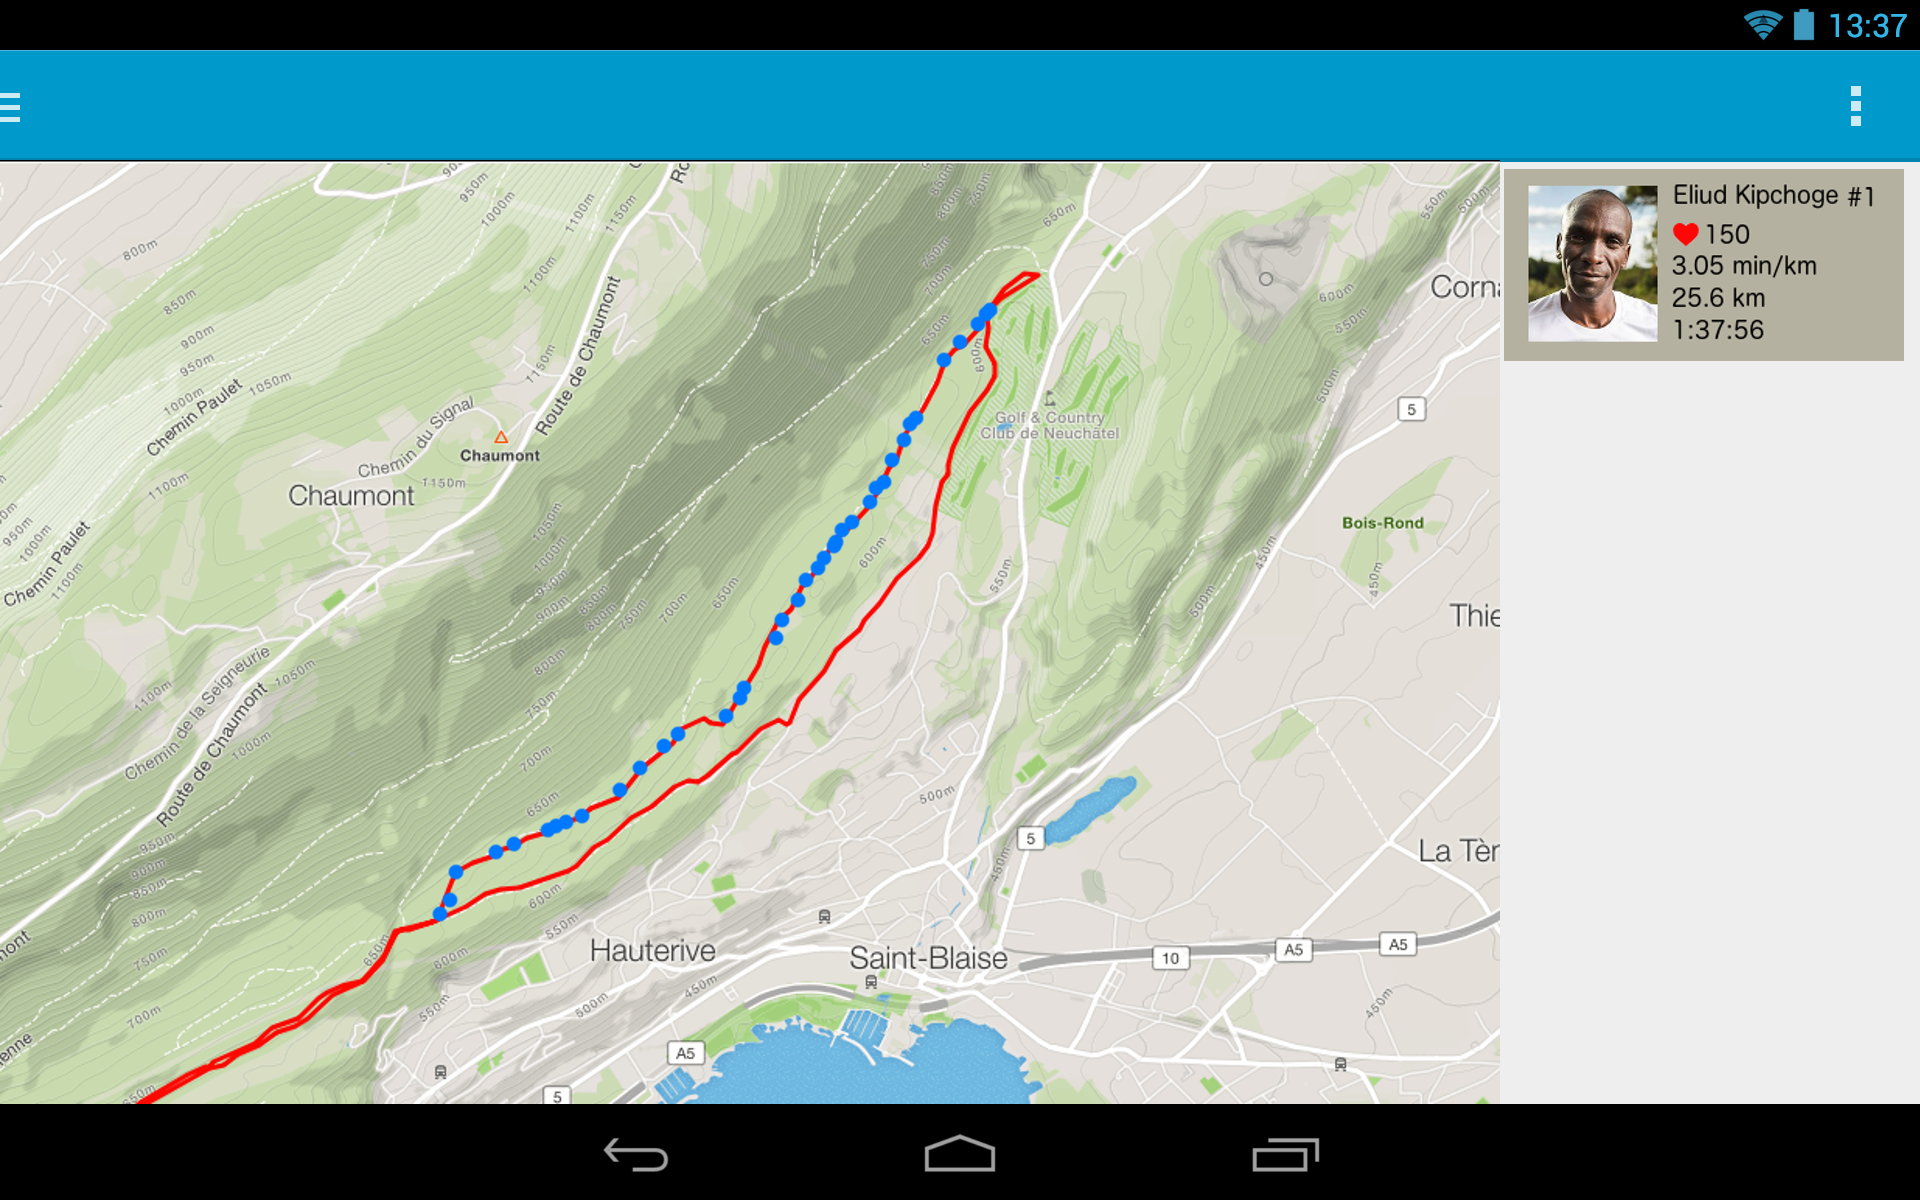
\includegraphics[width=0.8\columnwidth]{../images/app_mock.png} 
\caption[Concept application mobile]{Concept application mobile – Carte acquise depuis Strava}
\label{fig:esquisse_app}
\end{figure}

En plus de cela l’application proposera un menu de gestion des événements qui permettra à l’administrateur de la course d’effectuer diverses opérations de maintenances.

\begin{itemize}
\item Création de nouvelle course
\item Modification de course existante
\item Définition du parcours de la course
\item Ajout de coureur dans la base de données
\item Gestion de l’attribution des capteurs aux coureurs
\item Démarrage et fin d’une course
\end{itemize}

L'architecture générale de l'application mobile est décrite sur la figure~\ref{fig:archi_app}

\begin{figure}[htb]
\centering 
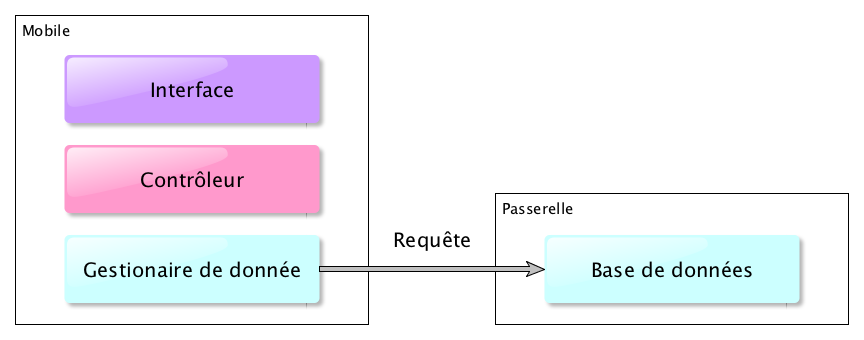
\includegraphics[width=0.8\columnwidth]{../images/archi_app.png} 
\caption[Architecture de l’application mobile]{Architecture de l’application mobile}
\label{fig:archi_app}
\end{figure}
